\documentclass[12pt, a4paper]{article}

\usepackage[utf8]{inputenc}
\usepackage{lmodern}
%\usepackage{fourier}
\usepackage{setspace}
	\singlespacing

\usepackage[frenchb]{babel}
\usepackage{xspace}
\usepackage[margin= 2.5cm]{geometry}
\pagestyle{plain}
\renewcommand{\thefootnote}{\fnsymbol{footnote}}

\usepackage{tikz}
	\usetikzlibrary{shapes}
\usepackage{graphicx}
	\graphicspath{{img/}}

\usepackage{varioref}
	\renewcommand{\reftextbefore}{page précédente}
	\renewcommand{\reftextfacebefore}{page ci-contre}
	\renewcommand{\reftextafter}{page suivante}
	\renewcommand{\reftextfaceafter}{page ci-contre}
	\renewcommand{\reftextcurrent}{}

\usepackage{amsmath, amsfonts}
\everymath{\displaystyle}


\newcommand{\espace}{\vspace{.8cm}}
\newcommand{\pg}{

}

%% REMPLIR
\usepackage[colorlinks=true, allcolors=blue, pdfborder={0 0 0}]{hyperref}
	\hypersetup{
		pdftitle={Défi Open},
		pdfsubject={Rapport Open},
		pdfkeywords={Open, IARISS, rapport},
		pdfauthor={IARISS Team}
	}
\title{Défi Open}
\newcommand{\authors}{Florent, Nicolas}

%
\begin{document}

\author{
\includegraphics{../_img/iariss_team.png} \\ {\sffamily \href{http://demo.iarissteam.me}{demo.iarissteam.me}}}
\date{\today}

\maketitle{}

{\sffamily Ce rapport a pour but de présenter rapidement la chartre graphique créée pour notre site web. Celle-ci utilise un framework CSS (\href{http://twitter.github.com/bootstrap/}{BootStrap Twitter}) qui permet l'utilisation avancée du CSS, du responsive design et le positionnement des éléments en fonction du navigateur et de la plateforme utilisés.} 

\espace{}
Pour commencer, voici la page d'accueil de notre application : 
\espace{}
\begin{center}
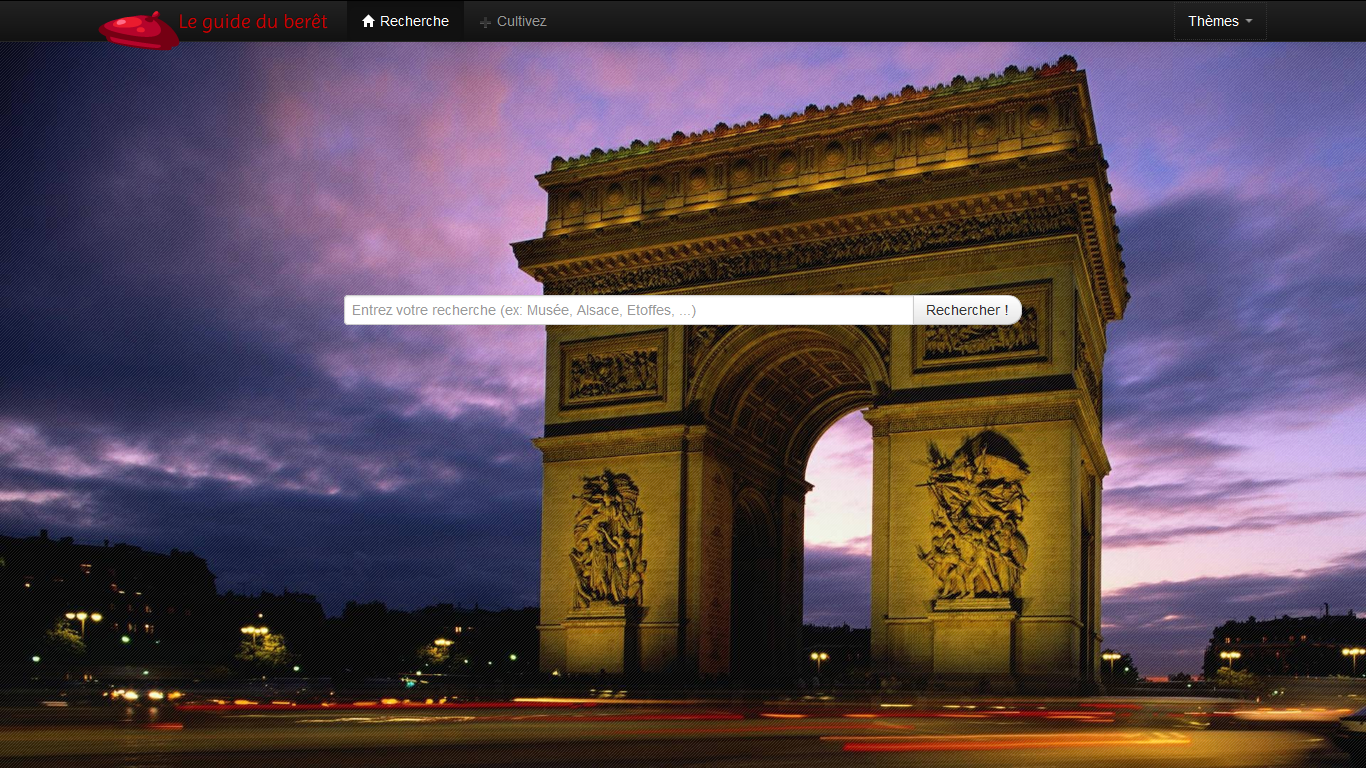
\includegraphics[width=.9\textwidth, keepaspectratio=true]{img/accueil.png}
\end{center}
\espace{}
Nous avons pris le parti de faire un design plutôt sobre et épuré : il est constitué d'une image de fond, par dessus laquelle est superposée de très légère rayure. La barre de navigation a été placée en haut de la fenêtre du navigateur, et la barre de recherche est centrée sur la page.

Trois onglets sont disponibles dans le menu de navigation : un onglet << Recherche >>, un onglet <<Cultivez >> et un onglet << Thèmes >>. Ce dernier permet de changer le thème de la page : en effet, plusieurs thèmes sont disponibles dans notre site web. Un changement de thème entraîne le changement de l'image de fond de l'application. Ci-après, exemple : 
\espace{}
\begin{center}
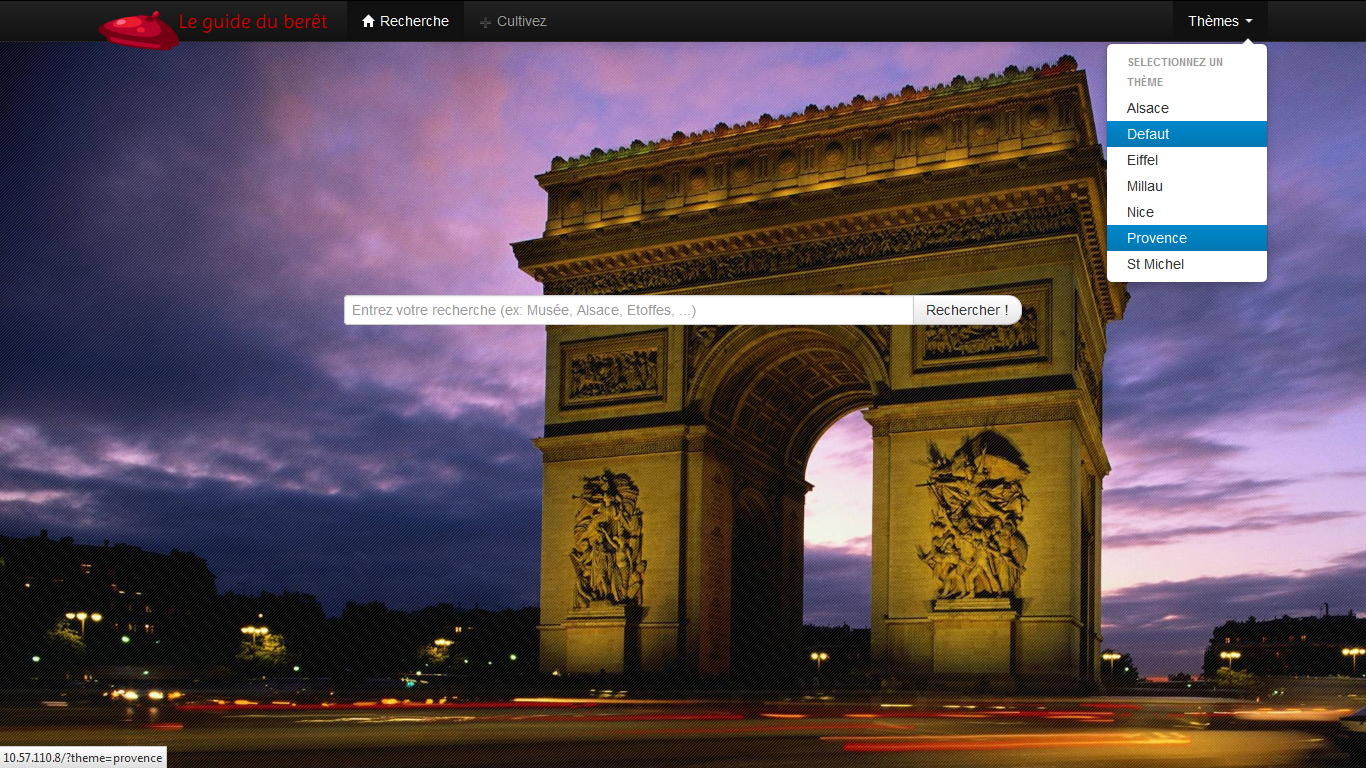
\includegraphics[width=.9\textwidth, keepaspectratio=true]{img/accueil3.png}
\espace{}
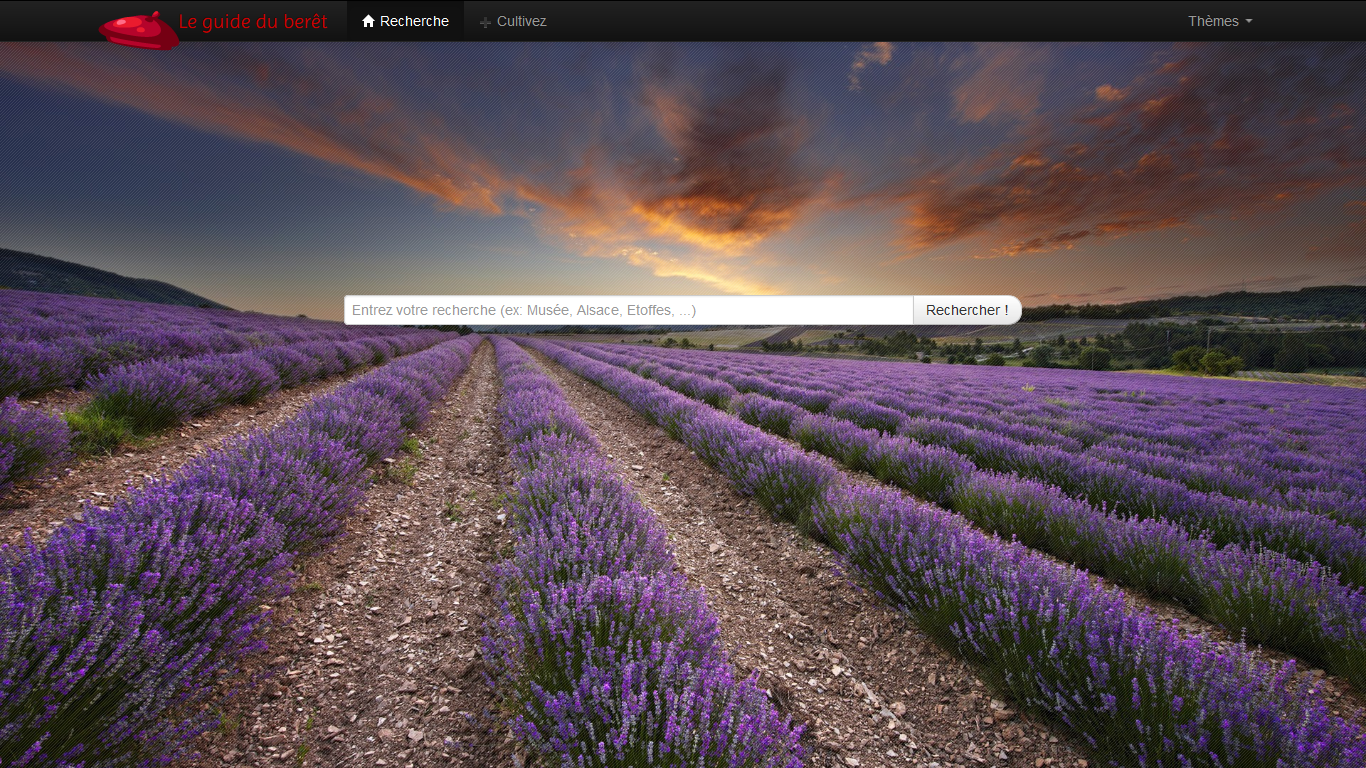
\includegraphics[width=.9\textwidth, keepaspectratio=true]{img/accueil2.png}
\end{center}

\espace{}
Intéressons nous aux deux autres onglets : << Recherche >> et << Cultivez >>.
Le premier onglet << Recherche >> permet d'afficher la page d'accueil de l'application, à savoir la barre de recherche qui permet à l'utilisateur d'entrer ses mots clés.

Le second, << Cultivez >>, permet à l'utilisateur d'ajouter du contenu sur le site : en effet, cette application étant en parti construit sur le principe d'un wiki, il faut que l'utilisateur puisse ajouter son propre contenu, et aussi l'éditer facilement.

Le site a aussi également été prévu pour s'adapter aux petites résolutions. En effet, le menu s'adapte automatiquement en fonction de la taille de la fenêtre. Voyons ceci plus en détails avec un exemple : dans les images qui suivent, nous avons volontairement réduit la taille de la fenêtre de notre navigateur.

\begin{center}
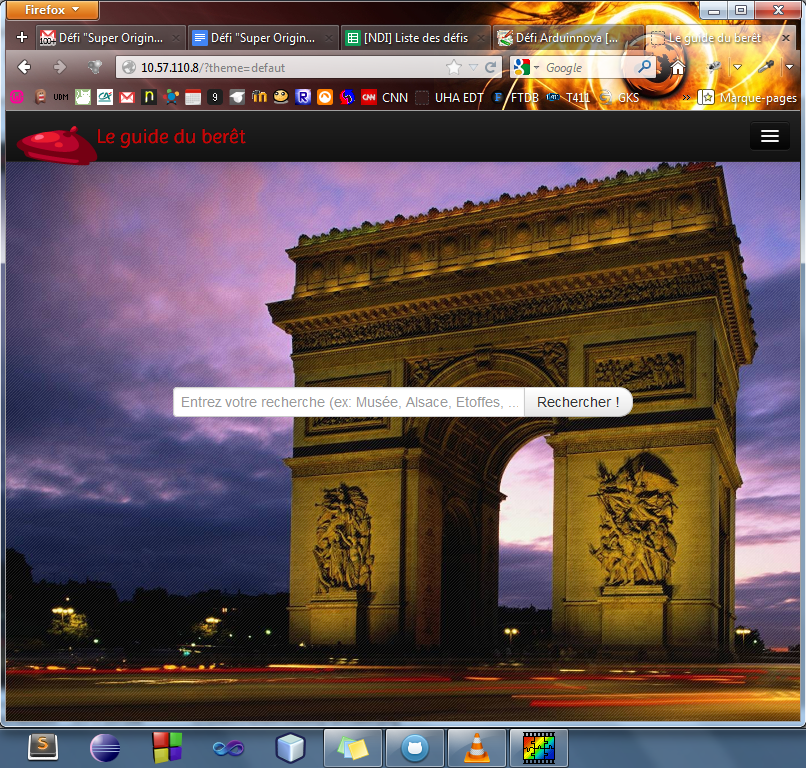
\includegraphics[width=.9\textwidth, keepaspectratio=true]{img/accueil4.png}
\end{center}

\espace{}
On voit déjà que les trois onglets ont disparu et qu'un autre est apparu. En cliquant dessus : 

\begin{center}
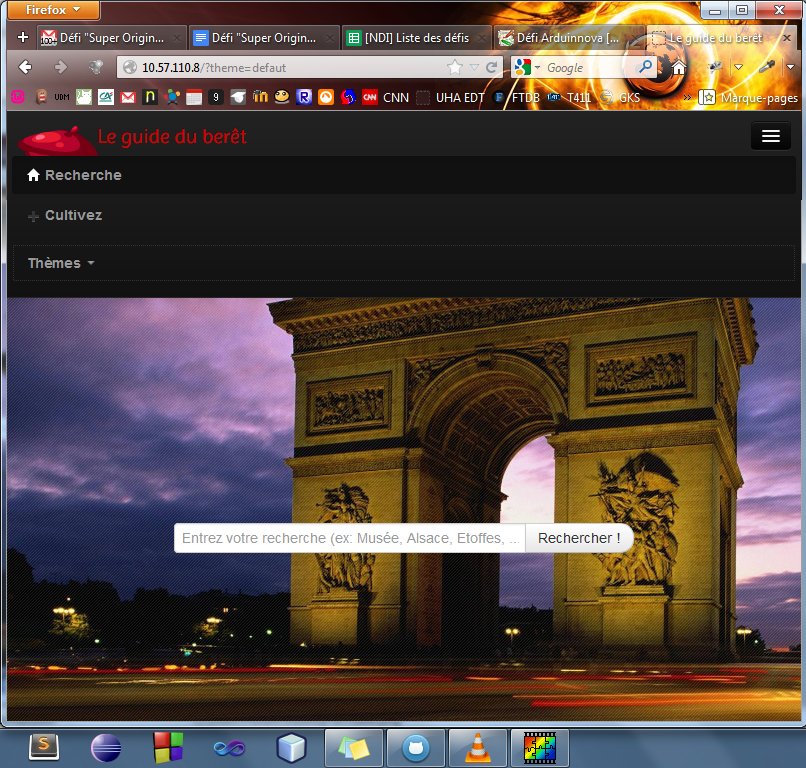
\includegraphics[width=.9\textwidth, keepaspectratio=true]{img/accueil5.png}
\end{center}

\espace{}
On s'aperçoit que l'on retrouve ici nos trois onglets. On peut également continuer à changer le thème, comme précédemment.

\espace{}
\espace{}
Vous trouverez la description de l'équipe sur \href{http://blog.iarissteam.me}{blog.iarissteam.me}.

\espace\vfill{}
Ce document a été rédigé en \LaTeX{} par \authors{} pour IarissTeam avec quelques tasses de café et beaucoup de bonne humeur.

Contactez-nous à \href{mailto:nuitinfo@iariss.com}{nuitinfo@iariss.com} pour tout renseignement supplémentaire !

\end{document}